%
% einleitung.tex -- Beispiel-File für die Einleitung
%
% (c) 2020 Prof Dr Andreas Müller, Hochschule Rapperswil
%
% !TEX root = ../../buch.tex
% !TEX encoding = UTF-8
%
\section{Die $\Gamma$-Funktion als Erweiterung der Fakultät\label{gamma:section:teil0}}
\kopfrechts{Fakultät erweitern}

Die Erweiterung der Fakultät beschäftigt grosse Namen der Mathematik schon lange.
Eine erste Definition der Fakultät für nicht natürliche Zahlen wird bereits 1720 von Daniel Bernoulli und Christian Goldbach gegeben.
Auch Leonhard Euler und James Stirling steuern im Laufe der Jahrhunderte ihre eigene Definition bei. 

\subsection{Bohr-Mullerup Theorem}

Um eine Funktion zu finden, welche die Fakultät erweitert, wird das Bohr-Mullerup Theorem verwendet.
Erfüllt eine Funktion Eigenschaften \eqref{gamma-eq:bm-1}, \eqref{gamma-eq:bm-2} und \eqref{gamma-eq:bm-3}, kann sie als Erweiterung der Fakultät für nicht natürliche Zahlen betrachtet werden.

\begin{equation}\label{gamma-eq:bm-1}f(1) = 1\end{equation}
\begin{equation}\label{gamma-eq:bm-2}f(x+1) = x \cdot f(x), x > 0\end{equation}
\begin{equation}\label{gamma-eq:bm-3}f(x) \text{ ist logarithmisch konvex}\end{equation} 

\noindent
Die Eigenschaft \eqref{gamma-eq:bm-1} ist selbsterklärend.
Die Eigenschaft \eqref{gamma-eq:bm-2} verlangt, dass die Funktion rekursiv definiert werden kann. 
Die Fakultät erfüllt das, da $5! = 5 \cdot 4!$ ist.
Die Eigenschaft \eqref{gamma-eq:bm-3} verlangt logarithmische Konvexität, was auch als ``wächst schnell'' verstanden werden kann.

\subsubsection{Logarithmische Konvexität}

Eine Kurve ist konvex, wenn diese wie in $f(x) = x^2$ nach oben geöffnet ist. 
Von logarithmischer Konvexität spricht man, wenn nach der Anwendung des Logarithmus, die resultierende Funktion auch konvex ist.
Gezeigt in Abb. \ref{gamma-fig:logConvex} anhand der Funktion $g(x) = e^{x^2}$.

\begin{equation}
  \label{gamma-eq:logConvex}
  g(x) = e^{x^2} \Rightarrow \ln(g(x)) = \ln\left(e^{x^2}\right) = x^2
\end{equation}

Die Funktion $x^2$ ist weiterhin nach oben geöffnet, womit $g(x)$ logarithmisch konvex ist.

\begin{figure}
  \centering
  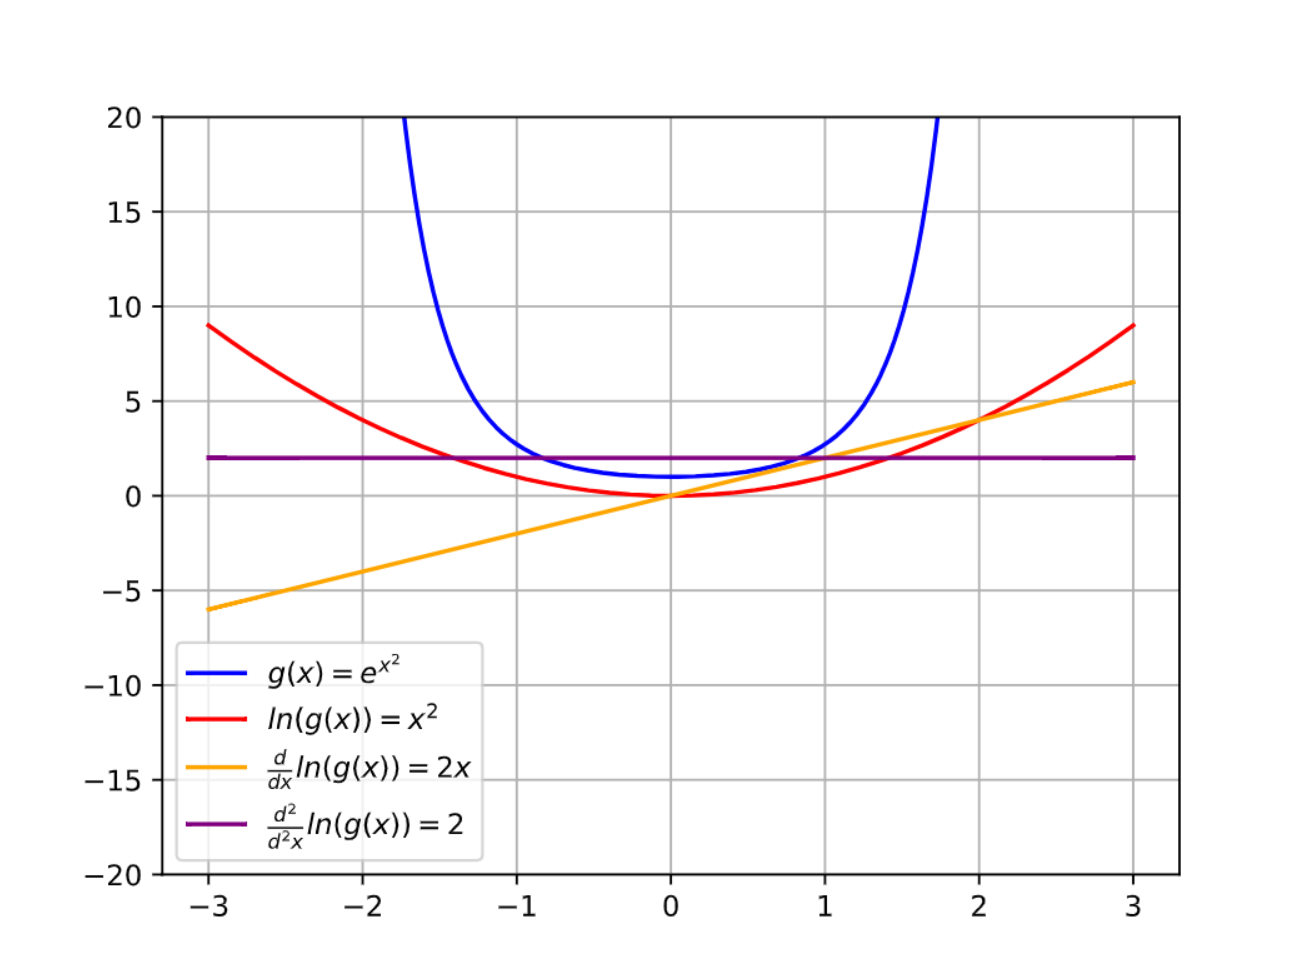
\includegraphics[width=0.6\textwidth]{papers/gamma/img/log_convex_3.png}
  \caption{Visualisierung der logarithmischen Konvexität von $g(x) = e^{x^2}$.}
  \label{gamma-fig:logConvex}
\end{figure}

\subsubsection{Suche nach einer passenden Funktion}

Eine Funktion welche Eigenschaften \eqref{gamma-eq:bm-1} und \eqref{gamma-eq:bm-2} erfüllt, lässt sich verhältnismässig leicht finden.
Als Beispiel, nimmt man die Funktion \eqref{gamma-eq:sinusFunction}, wird Eigenschaft \eqref{gamma-eq:bm-1} durch den Shift nach rechts und die \eqref{gamma-eq:bm-2} durch die Periode des Sinus erfüllt.

\begin{equation}
  \label{gamma-eq:sinusFunction}
  f(x) = 2\sin(2 \pi x)+1
\end{equation}

Wie die Grafik \ref{gamma-fig:almostGammaFunction} zeigt, geht \eqref{gamma-eq:sinusFunction} durch die bekannten Fakultät-Werte.
Die Ausschläge nach unten und oben zeigen grafisch, dass die logarithmische Konvexität \eqref{gamma-eq:bm-3} für diese Funktion nicht gegeben sein kann.

\begin{figure}
  \centering
  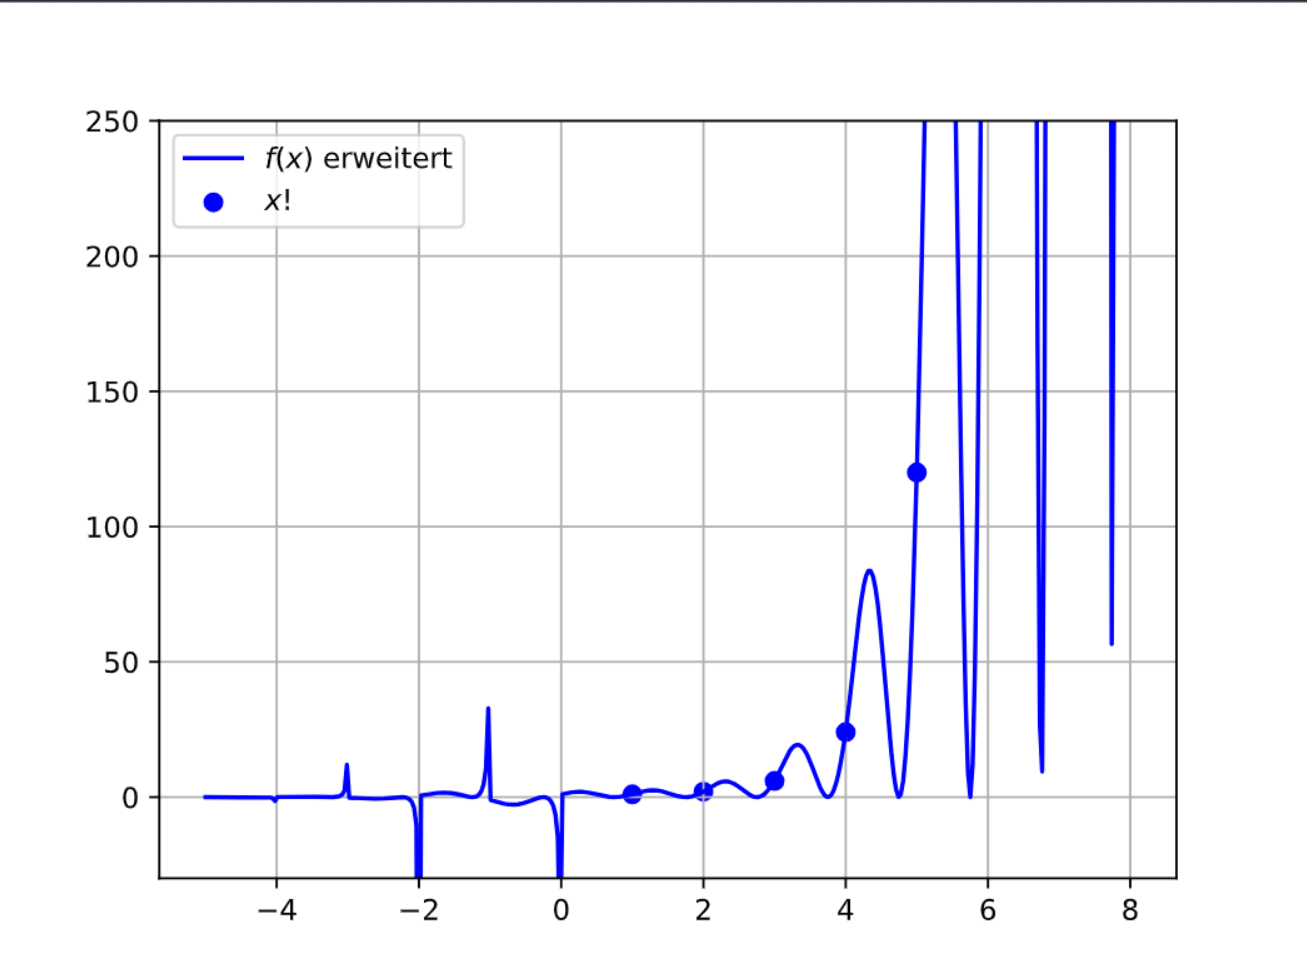
\includegraphics[width=0.6\textwidth]{papers/gamma/img/sin_extended.png}
  \caption{Funktion $f(x)$, welche zwei (\eqref{gamma-eq:bm-1} und \eqref{gamma-eq:bm-2}) von drei Eigenschaften erfüllt.}
  \label{gamma-fig:almostGammaFunction}
\end{figure}

Gesucht wird eine Funktion, welche alle Eigenschaften \eqref{gamma-eq:bm-1}, \eqref{gamma-eq:bm-2} und \eqref{gamma-eq:bm-3} der Fakultät respektive des Bool-Mullerup-Theorems erfüllt. 
Diese Herleitung ist nicht trivial und wird deshalb weggelassen. 
Lediglich die $\Gamma$-Funktion erfüllt alle Eigenschaften und ist somit die Erweiterung der Fakultät. 
